\begin{table}[t]
	\caption{\label{tab:timings}
		Per-iteration timing breakdown on \textsl{MipNeRF360} \cite{barron2022mip}.
		Our method significantly accelerates the ray tracing baseline.
	}
	\centering
	\small
	\begin{tabular}{c|c c}
		\toprule
		\textbf{Time} (ms) & \textbf{Total} & \textbf{Backward} \\
		\midrule
		% 3DGS & 10.8 & - & 20.6 \\
		% 3DGRT & 26.4 & 10.6 & 50.5 \\
		% %Ours & 18.4 & 7.7 & 18.0 \\
		% \textbf{Ours}\,(15spp) & 11.5 & 7.5 & 25.9 \\
		% \textbf{Ours}\,(30spp) & 23.3 & 7.7 & 28.9 \\
		3DGS               & \textbf{31.4}  & 20.6              \\
		3DGRT              & 87.5           & 50.5              \\
		%Ours & 18.4 & 7.7 & 18.0 \\
		% \textbf{Ours} (15spp) & 44.9 & 25.9 \\
		% \textbf{Ours} (30spp) & 59.9 & 28.9 \\
		\textbf{Ours}      & 39.8           & \textbf{17.9}     \\
		\bottomrule
	\end{tabular}
\end{table}


\section{Results}
\label{sec:results}
%
We evaluate our method against state-of-the-art baselines on standard benchmarks for both novel view synthesis and relightable reconstruction.

Our implementation builds on the 3DGRT codebase~\cite{loccoz20243dgrt}, using OptiX~\cite{optix} for hardware-accelerated ray tracing.
Sampling is performed in an OptiX \emph{any-hit} program, and the forward and backward passes run inside \emph{ray-gen} programs. Neural network evaluation and backpropagation use OptiX's Cooperative Vector interface~\cite{optix_coopvec}. All experiments are conducted on an Nvidia RTX 5880 Ada Generation GPU.

We set $\Mb=8$ backward samples for all experiments.
Since our stochastic algorithm tends to produce more Gaussians, we increase the densification interval to 400 in the novel view synthesis experiments to ensure a fair comparison.
Multiple forward samples are drawn via independent trials within a single BVH traversal for maximum efficiency; for relighting, we use $\Mf=15$.

By replacing sorted alpha blending with our stochastic estimator, we achieve substantially faster optimization with comparable visual quality on novel view synthesis benchmarks. Our method also naturally extends to relightable Gaussians, where accurate light transport estimation yields clear improvements over baselines.


\subsection{Novel View Synthesis}
\paragraph{Baselines}
Many recent works accelerate 3DGS optimization while preserving quality. Since our method only replaces the backward differentiation module, these techniques are largely orthogonal; we therefore compare against vanilla 3DGS and 3DGRT baselines.

For fair evaluation, all reconstructed scenes are rendered with 3DGRT's deterministic alpha blending.

\paragraph{Datasets}
We evaluate on four standard datasets: \textsl{MipNeRF-360} \cite{barron2022mip}, \textsl{Tanks \& Temples} \cite{Knapitsch2017}, \textsl{Deep Blending} \cite{DeepBlending2018}, and \textsl{NeRF Synthetic} \cite{mildenhall2020nerf}.

From \textsl{MipNeRF-360}, we select four indoor scenes (\textsl{room, counter, kitchen, bonsai}) and three outdoor scenes (\textsl{bicycle, garden, stump}).
From \textsl{Tanks \& Temples} we use \textsl{train} and \textsl{truck}; from \textsl{Deep Blending}, \textsl{playroom} and \textsl{drjohnson}.

\paragraph{Results}
Quantitative results are shown in \autoref{tab:benchmarks}. Our method delivers a substantial speed-up over 3DGRT while matching the speed of rasterization-based 3DGS, and achieves comparable reconstruction quality across all benchmarks. We test several forward sample counts in \autoref{tab:benchmarks} and adopt 30\,spp for the remaining experiments as the best speed--quality trade-off.

\autoref{fig:nvs_figures} presents an equal-time visual comparison: all methods run for the same wall-clock budget. \autoref{fig:psnr_vs_time} plots PSNR against optimization time, confirming that our method consistently converges faster than the sorted ray tracing baseline.

\begin{figure}[t]
	\centering
	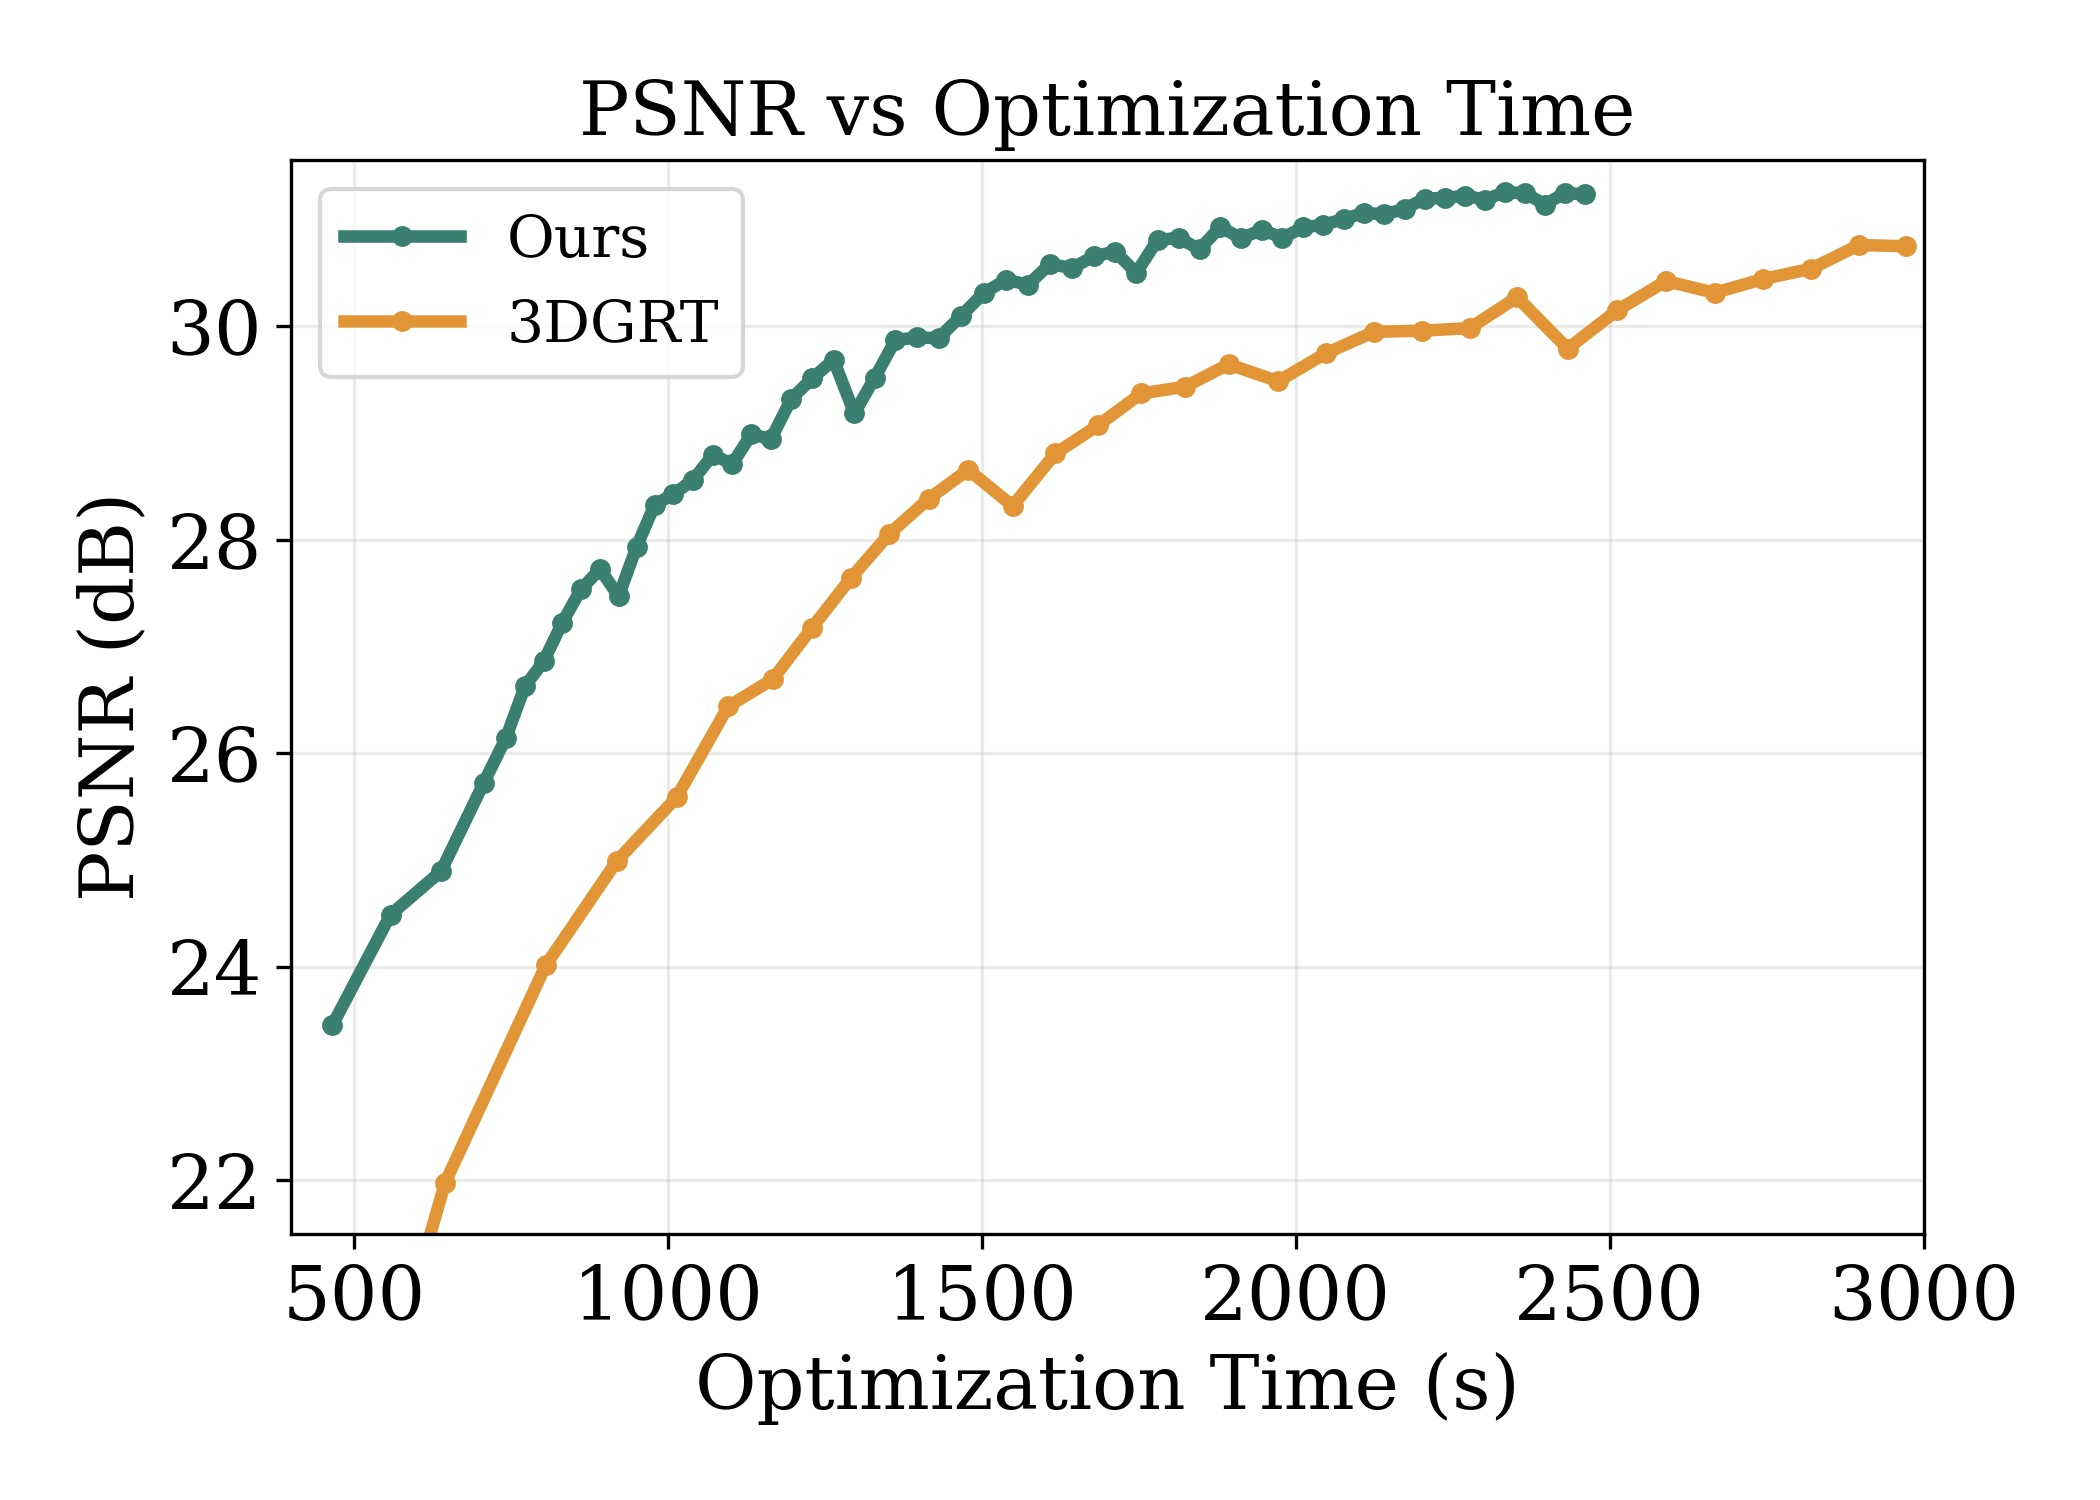
\includegraphics[width=0.8\linewidth]{images/psnr_curve_bonsai.jpg}
	\caption{\label{fig:psnr_vs_time}
		PSNR vs.\ optimization time for sorted alpha blending (3DGRT) and our method.
	}
\end{figure}


A per-stage timing breakdown appears in \autoref{tab:timings}.
Relative to 3DGS, our main overhead is BVH construction; relative to 3DGRT, our stochastic backward pass cuts iteration time by more than half.

% \begin{table}[]
%     \centering
%     \begin{tabular}{c|c c c c c}
%          & PSNR & SSIM & LPIPS & Train & FPS \\
%          \hline
%       3DGRT & 28.69 & 0.862 & 0.233 & 1h9m0s & \\
%       Ours & 28.34 & 0.852 & 0.251 & 43m40s & \\
%       Stoch-Splats & 24.67 & 0.714 & 0.392 & 1h23m23s&
%     \end{tabular}
%     \caption{Results of our method and baselines on MipNerf-360 Dataset}
%     \label{tab:placeholder}
% \end{table}


\begin{figure}[]
    \setlength{\resLen}{1.65in}
    %
    \centering
    \small
    \addtolength{\tabcolsep}{-5.5pt}
    %
    %
    \begin{tabular}{cc}
        % &
        (a) \textbf{Ours} & (b) \textbf{SS-Tracing}
        \\ \vspace{-0.1em}
        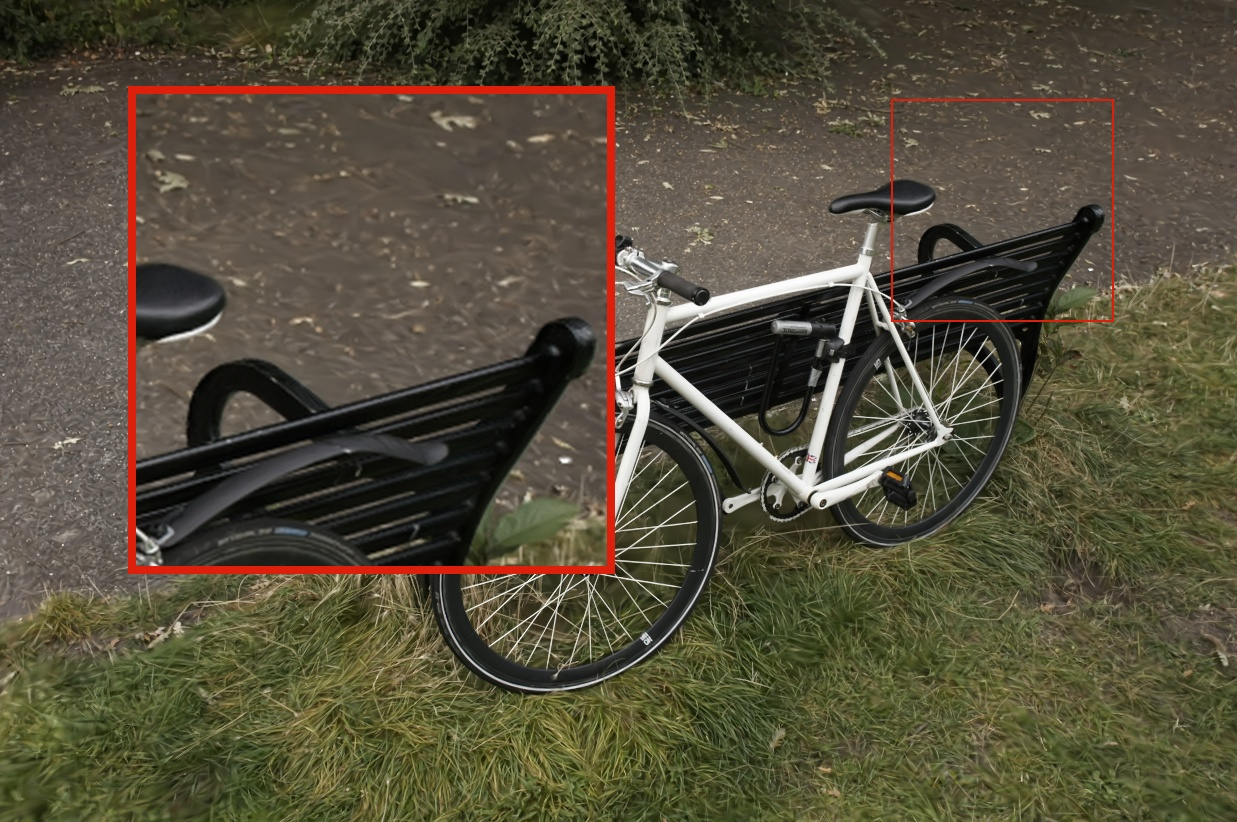
\includegraphics[width=\resLen]{images/nvs/bicycle/ours_30_composite.jpg} &
        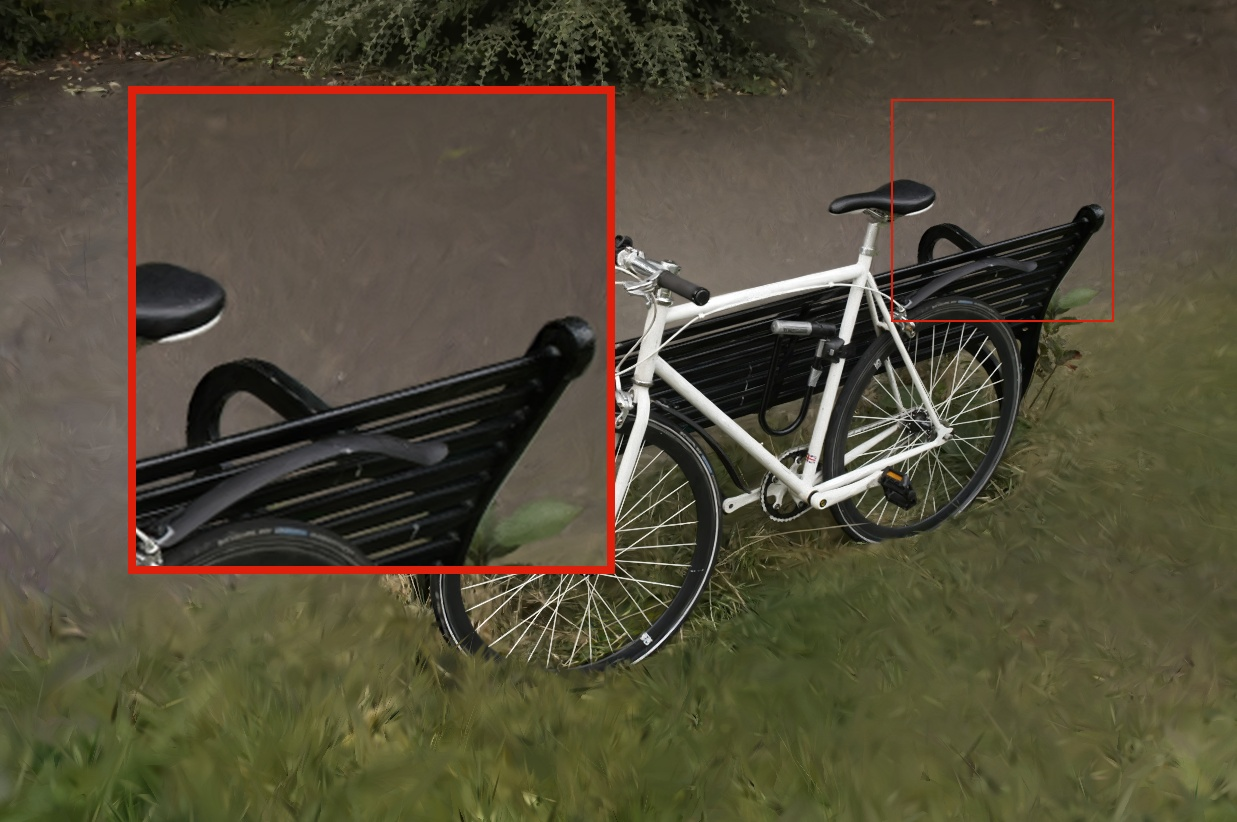
\includegraphics[width=\resLen]{images/nvs/bicycle/ssplats_composite.jpg} \\
        
\includegraphics[width=\resLen]{images/nvs/stump/ours_30_composite.jpg} &
        
\includegraphics[width=\resLen]{images/nvs/stump/ssplats_composite.jpg}
    \end{tabular}
    %
    \caption{
        Reconstruction quality comparison between our method and StochasticSplats~\cite{kv2025stochasticsplats}.
    }
    \label{fig:benchmark_ssplats}
\end{figure}
% \red{
	\paragraph{StochasticSplats comparison}
	We re-implement StochasticSplats in our ray tracing backend, denoting this variant \textsl{SS-Tracing}.
	\autoref{fig:benchmark_ssplats} compares novel-view synthesis results on the same datasets; quantitative metrics are reported in the appendix.
% }

\subsection{Relightable Gaussian Splatting}

\begin{table}[t]
	\caption{\label{tab:relightable_benchmarks}
		Results of our method and baselines on the \textsl{NRHints} dataset \cite{zeng2023nrhints}.
	}
	\centering
	\small
	\begin{tabular}{c|cccc}
		\toprule
		\footnotesize{PSNR$\uparrow$\;$|$\;SSIM$\uparrow$} & \textbf{Ours}                   & RNG                     & GS$^3$         \\
		\midrule
		\textsl{Lego}                                      & \textbf{30.40}$|$\textbf{0.949} & 26.72$|$0.924           & 26.62$|$0.923  \\
		\textsl{Basket}                                    & \textbf{28.02}$|$\textbf{0.956} & 19.97$|$0.853           & 23.22$|$0.936  \\
		\textsl{Pixiu}                                     & \textbf{30.89}$|$0.936          & 30.35$|$\textbf{0.941}  & 30.38$|$0.937  \\
		\textsl{Hotdog}                                    & \textbf{31.88}$|$0.955          & 30.38$|$\textbf{0.960}  & 25.40$|$ 0.949 \\
		\textsl{FurBall}                                   & \textbf{33.69}$|$\textbf{0.949} & 27.82$|$0.926           & 26.36$|$0.931  \\
		\textsl{Cat}                                       & \textbf{28.42}$|$0.870          & 28.39 $|$\textbf{0.888} & 26.09 $|$0.882 \\
		\bottomrule
	\end{tabular}
\end{table}

We compare against state-of-the-art relightable baselines RNG and GS$^3$.

Following RNG, we adopt a two-stage pipeline. Stage~1 optimizes the Gaussians as standard 3DGS with view-dependent spherical harmonics for 15,000 iterations to initialize geometry. Stage~2 switches to the neural appearance model of \autoref{Eq:neural_appearance} and fine-tunes for 85,000 iterations. The network has 4 hidden layers of dimension 64, and each Gaussian stores a 16-dimensional latent feature. Stage~1 hyperparameters match 3DGRT's novel view synthesis configuration; in Stage~2, densification, pruning, and density reset intervals are set to 3,000, 1,000, and 12,000 respectively, with all other settings unchanged.

We evaluate on the NRHints dataset~\cite{zeng2023nrhints}, consistent with the baselines. \autoref{tab:relightable_benchmarks} reports quantitative metrics; \autoref{fig:relightable_figures} visualizes reconstruction quality.

Because our pipeline traces exact shadow rays, it produces high-quality shadows and geometry without dedicated shadow-handling modules. As shown in \autoref{fig:relightable_figures}, this is consistently preferable to neural approximations.

\autoref{fig:environment_map_relighting} shows our reconstructions relit under novel environment maps. Despite training only with point-light illumination, the results are visually plausible---and our full ray-tracing pipeline incurs no additional overhead for environment lighting.
